

\section{Sparse Input processing}

%% methods deal with sparse input, like nconv, gconv ...
The depth map is supposed to be dense. Therefore, how to accept sparse depth map as input in CNNs is one of the most important problem. Some trivial solutions like median filters are good enough, if the missing pixels are sparse enough, however, for the case of huge missing holes in the depth map, it produces just a paltry result. Thus a reasonable guess is required for missing areas. Generally, it can be solved as image inpainting problems,\cite{inpainting1},\cite{inpainting2}. 

%% Deep learning based approaches
Some deep learning based method for image inpainting also achieved quite good performance for the hole mending task. 
%% talk about gconv
Notably, in 2016, Oord et al. \cite{gated_activation} proposed a gated activation unit for a CNN model,
\[\textbf{y} = \tanh (W_{k,f} * \textbf{x}) \odot \sigma (W_{k,g} * \textbf{x})\]
to substitute the standard activation layer, where $ \sigma $ is the sigmoid function, which constricts the output value of second part between $ [0,1] $.  The function is inspired by Long Short-Term Memory (LSTM) \cite{lstm} and Rated Recurrent Unit (GRU).\cite{gru} It is originally used for learning complex interactions as LSTM gates does. In 2018, Yu et al. \cite{gconv} employed same function for free-form image inpainting, which can be used to learn mask automatically from image it self.

%% talk about nconv
Different to aforementioned approaches, Knutsson et al. in 2005 introduced normalized convolution \cite{nconv} dealing with missing sample case for convolution operation, which aims to reconstruct the missing pixels from the sparse output sensed by cameras, which particularly considered the confidence of each interpolated pixels, since it provides the trustworthiness of the predicted value. The higher the reliability of the value inference, the better the model shape reconstruction.

In 2018, Eldesokey et al. \cite{ncnn} applied normalized convolution in CNN as normalized convolution layer that takes both sparse depth map and a binary confidence map as input to perform scene depth completion.
In 2020, Eldesokey et al. \cite{pncnn} focus on modeling the uncertainty of depth data instead of assuming binary input confidence.

\section{Normal Inference}



%% normal estimation method introduction
Ideally, the normal of each pixel in the depth map can be calculated based on its neighbor pixels constructing a over-determined function systems and solving by algebra methods\cite{geometry_based_solution}. This approach gives a quick but coarse normal inference. It also can be predict directly by feeding the image directly into a CNN \cite{Eigen}, in this case, no depth map is required.
GeoNet\cite{GeoNet} integrates both ideas to refine the coarse normal map with another CNN predicted normal map. 
%% traditional methods

In 2012, Holzer et al. \cite{Holzer.S} presented a read-time method, which is able to run algorithm in a high frame speed. They smooth the depth data in order to handle the noise of depth image. The speed is accelerated via integral image. The drawbacks are, as mentioned in the paper, the normals error go up when point depths change severely.

In 2018, Yu et al. \cite{gconv} presented a CNN based method with gated convolutional layer.

In 2018, Hua et al. \cite{guided} presented an approach integrating color image and certainty map into the network to enhance the performance of depth map density.

In 2019, Ben-Shabat et al. \cite{Ben-Shabat_2019_CVPR} presented a CNN based method.

In 2021, Zhou et al.  \cite{zhou2021fast}

%% CNN based methods
The deep convolutional neural network is typically used for image classification, which achieved great success in last several years. \cite{yolov3}, \cite{efficientDet}.

%% talk about the reason we need new type of network architecture
These kinds of network architecture takes a single image as input which usually employed for classification problems. The image is usually convoluted with convolutional layer and downsampling with pooling layers. The outputs of the network consists of a single value to represent the ID of corresponding class \cite{efficientDet}, or with set of values to represent the position of bounding boxes.\cite{yolov3}.

However, in many other vision tasks, the output is demanded as an image, instead of predicting one or several classes of the input, but the classes of each pixel are predicted. In this case, the traditional network architecture is not suitable anymore.

%% talk about image upsampling, unet
Recently, Ronneberger et al proposed an architecture called UNet \cite{unet} for biomedical image segmentations. The architecture is shown in Figure \ref{fig:u-net}.The first half network is a usual classification convolutional network, the second half replace the pooling layers to upsampling layers, thus in the end of the second half, the output is back to the input size. The proposed network can successfully assigned each pixel a class for segmentation tasks. Under this symmetric network, an input image is downsampled 3 times and upsampled 3 times. Output image has exactly the same size as input image. The downsampling and upsampling both have large number of feature channels, which guarantee the network propagates the information to higher resolution layers.


\begin{figure}[!h]
	\centering
	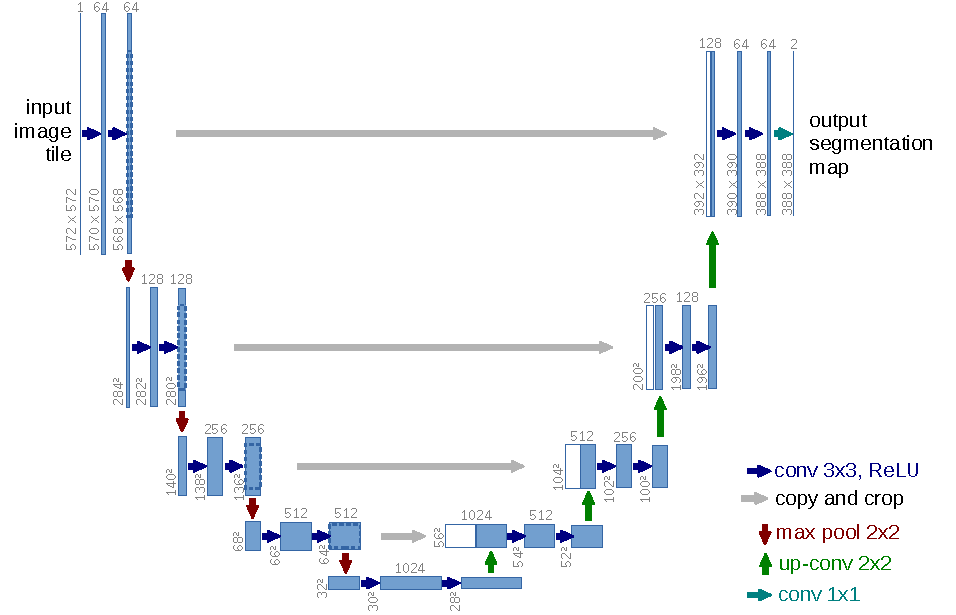
\includegraphics[width=\textwidth]{./ref/u-net-illustration-correct-scale2}
	\caption{U-net architecture (example for 32x32 pixels in the lowest resolution). Each blue box corresponds to a multi-channel feature map. The number of channels is denoted on top of the box. The x-y-size is provided at the lower left edge of the box. White boxes represent copied feature maps. The arrows denote the different operations.
	}
	\label{fig:u-net}
\end{figure}





%% guided scene completion






